\documentclass[review]{elsarticle}
\usepackage{comment}
\usepackage{url}
%
\usepackage[breaklinks]{hyperref}
\usepackage{breakurl}


\usepackage[ruled]{algorithm2e}

%\usepackage{lineno}
%\modulolinenumbers[5]

\journal{Optics Communications}

%%%%%%%%%%%%%%%%%%%%%%%
%% Elsevier bibliography styles
%%%%%%%%%%%%%%%%%%%%%%%
%% To change the style, put a % in front of the second line of the current style and
%% remove the % from the second line of the style you would like to use.
%%%%%%%%%%%%%%%%%%%%%%%

%% Numbered
%\bibliographystyle{model1-num-names}

%% Numbered without titles
%\bibliographystyle{model1a-num-names}

%% Harvard
%\bibliographystyle{model2-names.bst}\biboptions{authoryear}

%% Vancouver numbered
%\usepackage{numcompress}\bibliographystyle{model3-num-names}

%% Vancouver name/year
%\usepackage{numcompress}\bibliographystyle{model4-names}\biboptions{authoryear}

%% APA style
%\bibliographystyle{model5-names}\biboptions{authoryear}

%% AMA style
%\usepackage{numcompress}\bibliographystyle{model6-num-names}

%% `Elsevier LaTeX' style
\bibliographystyle{elsarticle-num}
%%%%%%%%%%%%%%%%%%%%%%%
\usepackage{graphicx}
\usepackage{subcaption}
%%%%%%%%%%%%%%%%%%%%%%%%%%%%%%%%%%%%%%%%%%%%%%%%%%%%%%%%%%%%%%%%%%%%%%%%%%%%%%%%%%

\usepackage[svgnames]{xcolor} % Enabling colors by their 'svgnames'

\usepackage{amsmath}
\usepackage{amsfonts}
\usepackage{amssymb}
%%%%%%%%%%%%%%%%%%%%%%%%%%%%%%%%%%%%%%%%%%%%%%%%%%%%%%%%%%%%%%%%%%%%%%%%%%%%%%%%%%

 
\begin{document} 

\begin{frontmatter}

\title{Sampling Frequency in the Dynamic Speckle Analysis}
%\tnotetext[mytitlenote]{Fully documented templates are available in the 
%elsarticle package on \href{http://www.ctan.org/tex-archive/macros/latex/contrib/elsarticle}{CTAN}.}



% Group authors per affiliation:
\author{Rivera, F. P.}
\author{Pe\~na, R. G.}
\author{Braga, R. A.}



\address{University Federal of Lavras, Lavras, Brazil}
%\fntext[myfootnote2]{201518201@posgrad.ufla.br}
%\fntext[myfootnote1]{robertobraga@deg.ufla.br }
% 


\begin{abstract}
In this article, we show as the variation of sampling frequency, 
in a dynamic speckle analysis, affects the value of some dynamic speckle index, 
to the cases of the absolute value of the differences index, the temporal 
speckle standard deviation index and the temporal 
speckle mean index.
We show that  the dynamic speckle index value change the maximum excursion with 
the variation of sampling frequency, affected directly by the time integration 
(exposition time) of camera.
We highlight the importance of knowing  the frequency band of analyzed phenomenon, 
in order to choose the appropriate sampling frequency, 
being recommendable to use the minimal sampling frequency possible
to get an acceptable maximum excursion, 
and an illumination level with good signal-noise ratio.

\end{abstract}

\begin{keyword}
Sampling frequency \sep
Dynamic speckle index \sep 
Dynamic speckle index \sep 
Dynamic speckle analysis
\end{keyword}

\end{frontmatter}

\linenumbers


%%%%%%%%%%%%%%%%%%%%%%%%%%%%%%%%%%%%%%%%%%%%%%%%%%%%%%%%%%%%%%%%%%%%%%%%%%%%%%%%
%%%%%%%%%%%%%%%%%%%%%%%%%%%%%%%%%%%%%%%%%%%%%%%%%%%%%%%%%%%%%%%%%%%%%%%%%%%%%%%%
%%%%%%%%%%%%%%%%%%%%%%%%%%%%%%%%%%%%%%%%%%%%%%%%%%%%%%%%%%%%%%%%%%%%%%%%%%%%%%%%
%%%%%%%%%%%%%%%%%%%%%%%%%%%%%%%%%%%%%%%%%%%%%%%%%%%%%%%%%%%%%%%%%%%%%%%%%%%%%%%%
\section{Introduction}


%1) Anuncie o tema e o problema do artigo (forma de pergunta + definiçoes)
The dynamic laser speckle analysis is  an important
study topic\cite{catalano2019viability,rivera2019sound,gonzalez2018diode,Silva2018,braga2017dynamic} 
to determine the  activity level of biological materials. 
The importance of technical aspects of dynamic laser speckle analysis,
as the stability of laser illumination level has been  analyzed \cite{gonzalez2018diode}, 
and it was analyzed the effect of illumination instability over an index value \cite{gonzalez2018diode},
such as the absolute values of the differences \cite{cardoso2014,rivera2017selection}.
It  was showed the dependence between the index value and the illumination level. 

%3) Resgate a problematica( Importancia do problema de pesquisa - extenda primer passo)
Thus, 
it is necessary analyze the effect of technical parameters that affect the perceived illumination level; 
in these sense,
we analyze the effect of sampling frequency, 
and consequently the time exposure, in a dynamic laser speckle analysis
that use: the absolute value of the differences index, 
the temporal speckle standard deviation index and the temporal speckle mean index \cite{Nothdurft:05}. 

%4) Relevancia do artigo(importancia para outros del artigo publicado)
Knowing the effect of sampling frequency over an index value,
a researcher will be able to have a criteria to choose the appropriate sampling frequency 
for a certain monitored phenomenon. 
% Thus,
% optimizing resources when choosing the hardware specification in a system setup; 
% being in this case, the limitations relatives to illumination level and signal-noise relation in the study sample.

%5) Anuncie a hipotesis
For this purpose, we show that given a dynamic speckle test, exists an appropriate frequency band
to the sampling frequency. High values of sampling rate may cause unintended consequences on the index value, 
such as the decrease of the excursion between two activity levels, given a determinate index value. 
In turn, decreasing the sampling frequency promoted by the increasing of the exposure time,
will cause a reduction of the temporal speckle contrast,
 and consequently limit the possibility  to get information from the sample.  

%6) Anuncie os objetivos (receita pra demostrar a h.)
To be able to demonstrate the existence of this appropriate frequency band,
we will perform two types of tests; in the first, we analyzed an ink drying process along the time; and in
the second, we tested the activity state of a corn seed, with 3 days of germination.
In both cases, were used four different sampling rates, 
and was compared the behavior of speckle indexes.

%2) Exponha qual será o percurso (defina seçoes)
In the next section we describe how the speckle images were acquired and the setup used to analyze them; 
all theoretical definitions, necessary to understand the analysis, will shown in the Section 3;
numerical results of the analysis  are presented in Section 4, and
an analysis of the results is reported in the Section 5; finally, we present our
conclusion in the Section 6.

%%%%%%%%%%%%%%%%%%%%%%%%%%%%%%%%%%%%%%%%%%%%%%%%%%%%%%%%%%%%%%%%%%%%%%%%%%%%%%%%
%%%%%%%%%%%%%%%%%%%%%%%%%%%%%%%%%%%%%%%%%%%%%%%%%%%%%%%%%%%%%%%%%%%%%%%%%%%%%%%%
%%%%%%%%%%%%%%%%%%%%%%%%%%%%%%%%%%%%%%%%%%%%%%%%%%%%%%%%%%%%%%%%%%%%%%%%%%%%%%%%
%%%%%%%%%%%%%%%%%%%%%%%%%%%%%%%%%%%%%%%%%%%%%%%%%%%%%%%%%%%%%%%%%%%%%%%%%%%%%%%%
\section{System description}
\label{sec:description}




\subsection{Time exposure of the camera}
\label{subsec:expositiontime}
The sampling frequency ($F_s$) or acquisition time in frames per second ($fps$), 
in the camera Marlin F-033 is obtained using the 
 Table \ref{table:1}, 
\begin{table}[h!]
\centering
\begin{tabular}{||c c c c c||} 
 \hline
 $Shutter$ &  $Base$ [$\mu s$] & $Offset$ [$\mu s$] & $E$ [$ms$] & $F_s$ [$fps$]\\ [0.5ex] 
 \hline\hline
 3332  & 20  & 12  & 66.652  & 15.003  \\ 
 1665  & 20  & 12  & 33.312  & 30.019  \\ 
 1110  & 20  & 12  & 22.212  & 45.021  \\ 
 832   & 20  & 12  & 16.652  & 60.053  \\ [1ex] 
 \hline
\end{tabular}
\caption{Exposition time and sampling frequency}
\label{table:1}
\end{table}
where we can see the 4 sampling frequencies that will be used in the tests;
these values were obtained using  
the shutter register value ($Shutter$), 
the time base register value ($Base$),
the exposure time offset ($Offset$) and
the effective exposure time ($E$);
 so that the exposure time ($Exposure$),
\begin{equation}
Exposure= Shutter \times Base,
\end{equation}
\begin{equation}
\frac{1}{F_s}=E= Exposure + Offset.
\end{equation}
Where,  $F_s$ is calculated in relation to $E$; being that,
the $Exposure$ represent the photography integration time and $E$ the effective time
between photographs; 
the difference between these two exposures arise from $Offset$ time, 
that is the time between end and start of a photography.
In all cases the exposure time is much bigger than $Offset$; so, we can approximate
that $F_s\approx 1/Exposure$.


\subsection{Data-packages of ink drying process}
\label{subsec:data1}
 This data set comes from an ink drying process, 
 where groups of images (data package) are taken at the times
 $\{0,$ $1,$ $2,$ $3,$ $4,$ $5,$ $6,$ $7,$ $8,$ $9,$ $10\}$ min. 
 In each time, an acquired package  has 512 images of 147 pixels of height and 166 pixels of width.
4 different sampling rates were used to take the images,
 being these rates $15$, $30$, $45$ and $60$ hz.

\subsection{Data-package of maize seed germination}
\label{subsec:data2}
 This data-package has the speckle pattern of a maize seed with 3 days of germination,
 where four data-packages with different sampling rates ( $15$, $30$, $45$ and $60$ hz)  
were built.
Each package have 512 images of $15$ pixels of height and $15$ pixels of width.
 

\subsection{Test 1: ink drying process}
\label{subsec:test1}
Fig. \ref{fig:test1} represents the data analysis method in an ink drying process, 
to a $F_s$ sampling rate.
\begin{figure}[ht!]
\centering
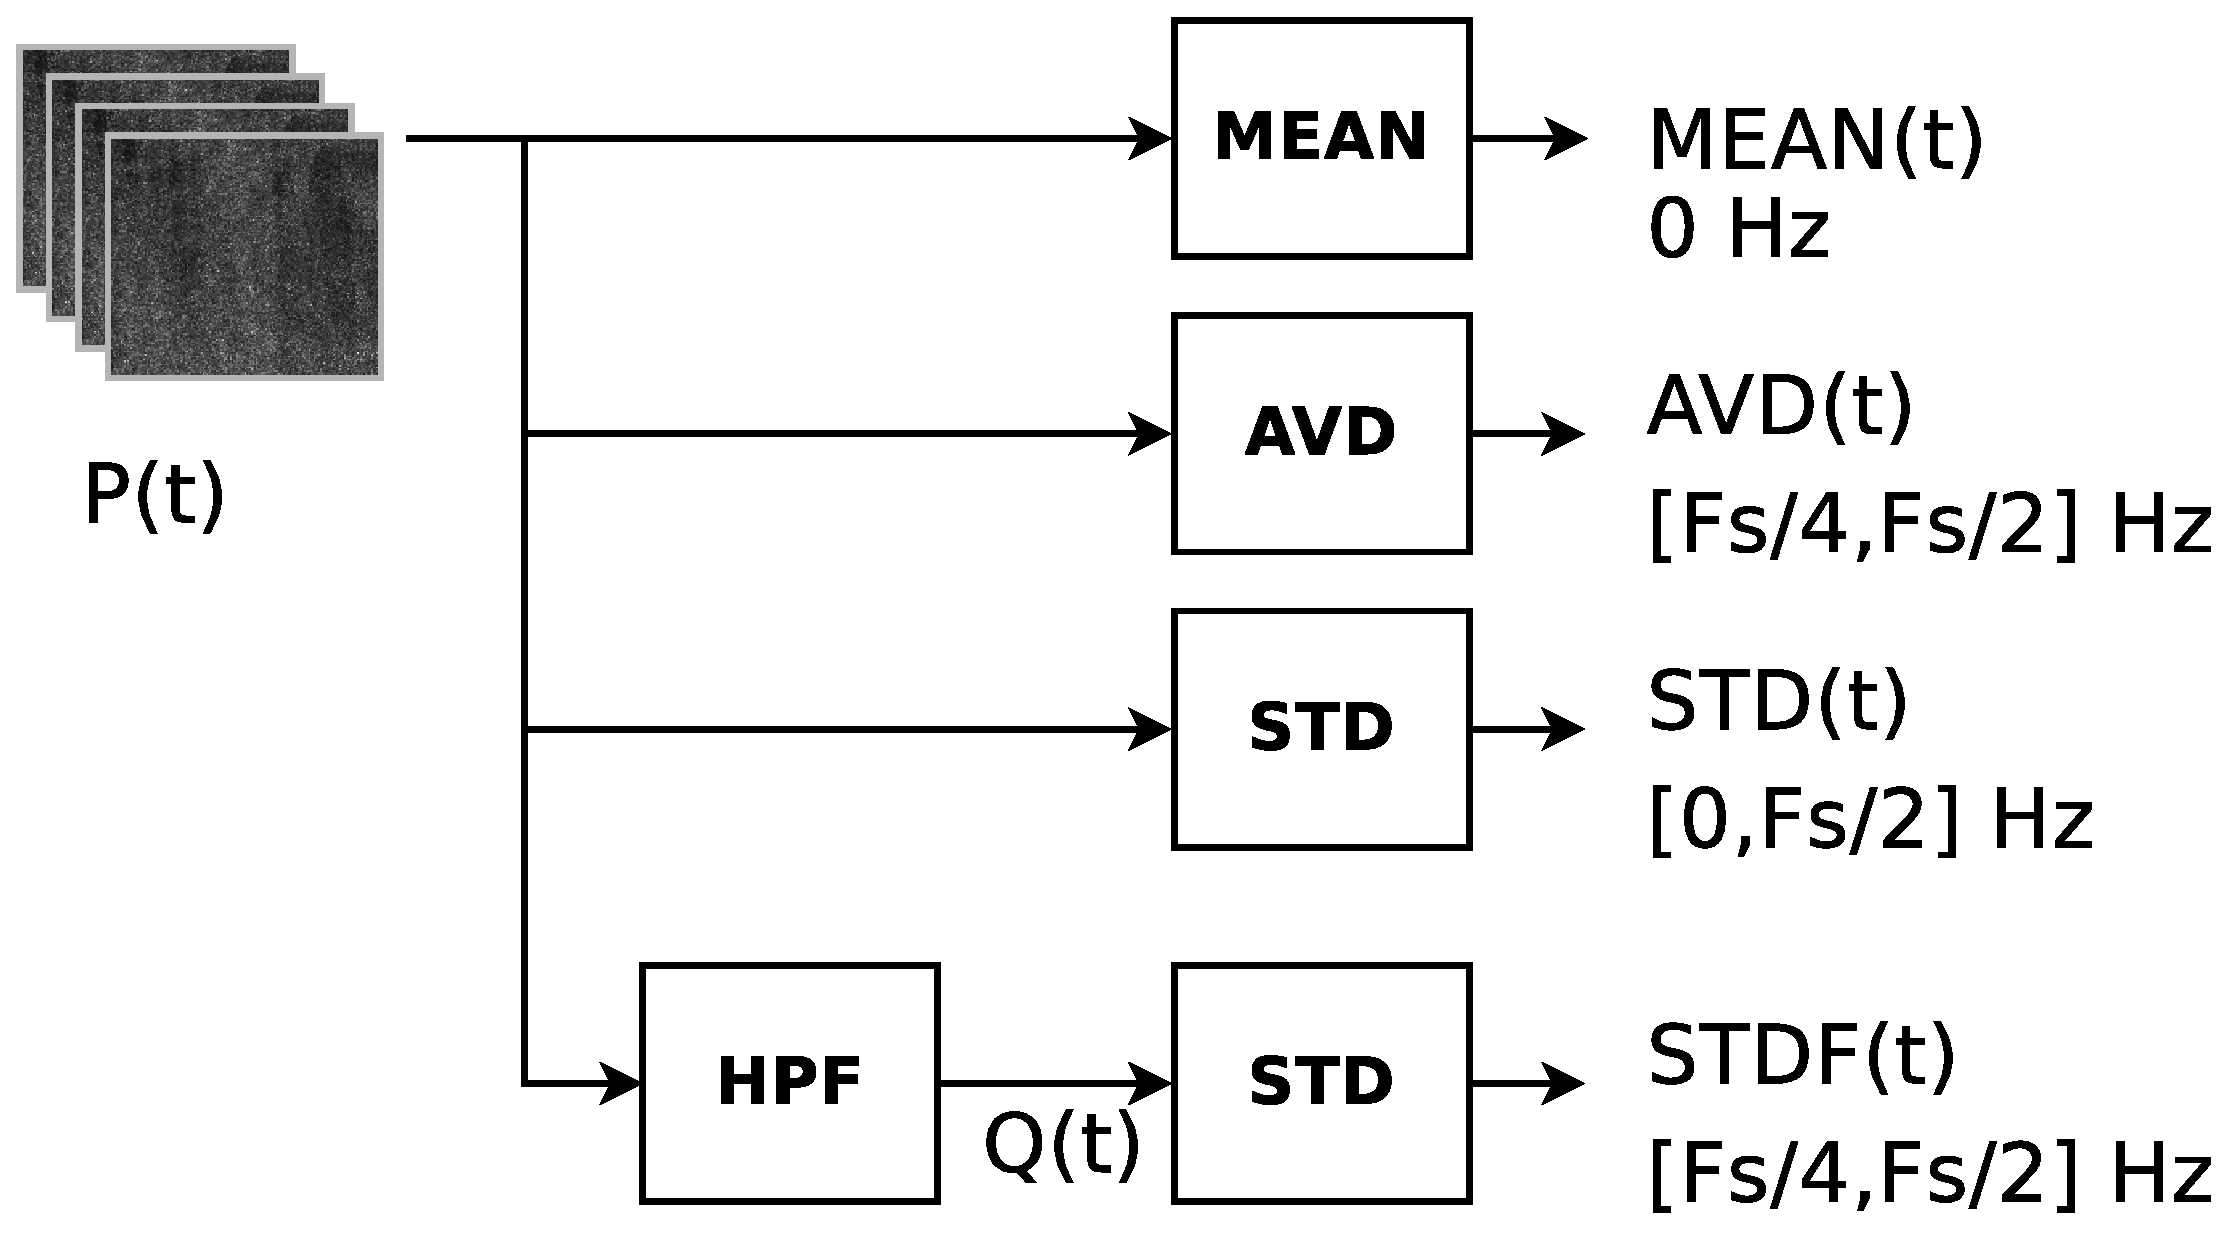
\includegraphics[width=0.55\columnwidth]{test1.eps}
\caption{Data analysis of the ink drying process test.}
\label{fig:test1}
\end{figure}
Where, $P(t)$ is an data-package with  images at the time $t$ minutes; 
this package has $N$ images and $M$ pixels; $P_{n,m}(t)$ 
define the $n$-th image and $m$-th pixel, for all $1 \leq n \leq N$, $1 \leq m \leq M$.
The $MEAN$ block represents the calculation of temporal speckle mean index on 
the package $P(t)$, returning the value $MEAN(t)$. 
The $AVD$ block represents the calculation of  absolute values of the differences index on
the package $P(t)$, returning the value $AVD(t)$. 
The $STD$ block represents the calculation of the temporal speckle standard deviation index on 
the package $P(t)$ or $Q(t)$, returning the value $STD(t)$ or $STDF(t)$, respectively.
And finally,
the block \hyperref[sec:stdf]{$HPF$} represents a digital finite impulse response ``high-pass filter'' 
with order $40$ and cut-off at $0.25F_s$; this block filter the $P(t)$ package and return $Q(t)$,
leading this result to a $STD$ block to finally obtain the $STDF(t)$ index value.
According to the information of the data packages, 
we will have speckle indexes values, for each minute, during 10 minutes.

\subsection{Test 2: Maize seed germination}
\label{subsec:test2}
The speckle activity of a maize seed
was analyzed in a similar way to the ink drying, seen in the Section \ref{subsec:test1}, 
with the difference that only one data-package was taken at the time $t$, equal to 3 days of germination.

\subsection{Test 3: Frequency band activity analysis}
\label{subsec:test3}

The Fig. \ref{fig:test3} represents the frequency band analysis method of data package $P$, 
acquired  with a sampling rate of $F_s$. This package is the input of many band pass filter (\hyperref[sec:stdb]{$BPF$}) blocks,
described in the Sec \ref{sec:stdb}, these band pass filter have cut-off frequencies between $f_1(l)$ and $f_2(l)$,
where $l$ indicates the current band, so that $1\leq l\leq L$;
being $L$ the total number of analysis frequency bands; 
thus, we obtained the  $R_l$ package (a filtered version of $P$). $R_l$ was processed 
by a $\sigma$ block, where it is calculated the $\sigma_{m}$ value to each pixel in the package $R_l$,
as described in the Sec \ref{sec:std}. Finally, 
an image is obtained and it is named as the variable $STDB_l$.
\begin{figure}[ht!]
\centering
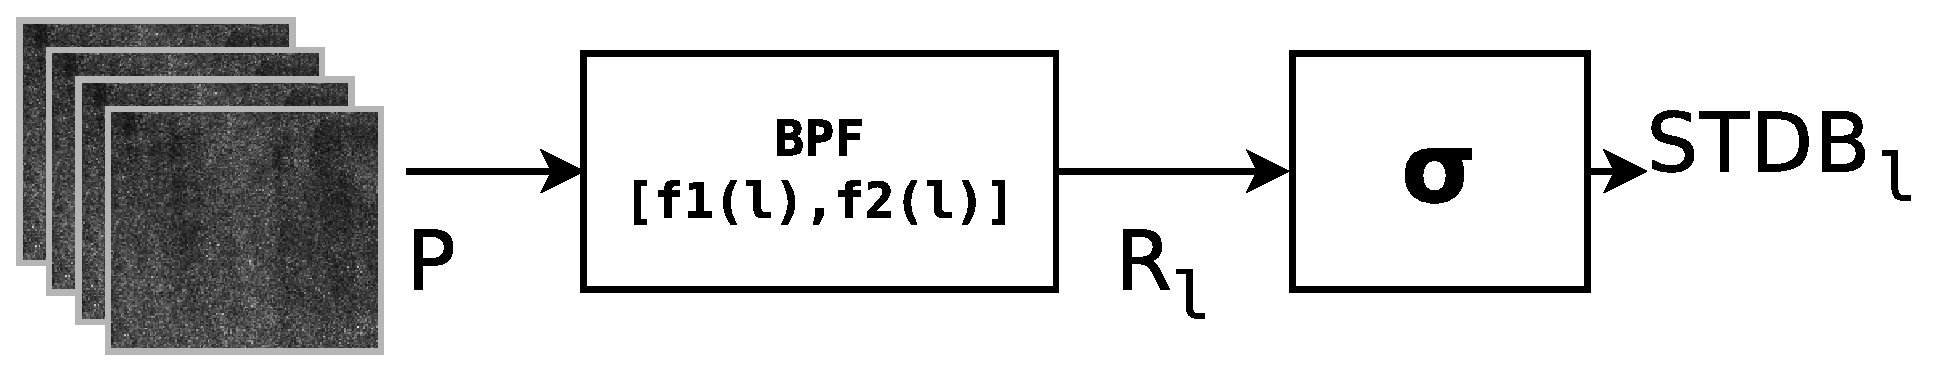
\includegraphics[width=0.55\columnwidth]{test3.eps}
\caption{Frequency band analysis of a data package.}
\label{fig:test3}
\end{figure}

 

%%%%%%%%%%%%%%%%%%%%%%%%%%%%%%%%%%%%%%%%%%%%%%%%%%%%%%%%%%%%%%%%%%%%%%%%%%%%%%%%
%%%%%%%%%%%%%%%%%%%%%%%%%%%%%%%%%%%%%%%%%%%%%%%%%%%%%%%%%%%%%%%%%%%%%%%%%%%%%%%%
%%%%%%%%%%%%%%%%%%%%%%%%%%%%%%%%%%%%%%%%%%%%%%%%%%%%%%%%%%%%%%%%%%%%%%%%%%%%%%%%
%%%%%%%%%%%%%%%%%%%%%%%%%%%%%%%%%%%%%%%%%%%%%%%%%%%%%%%%%%%%%%%%%%%%%%%%%%%%%%%%
\section{Theoretical definitions}
\label{sec:theoretical}

In the next subsections we use the variable $P$ to define $P(t)$ in any time $t$;
thus, $P$ represents a data collection of images in any time.

\subsection{$MEAN$ index }
\label{sec:mean}

The temporal speckle mean index ($\mu_{m}$) \cite{Nothdurft:05} gives the mean
value of the illumination level to the $m$-th pixel in the package $P$, 
and it was  implemented as presented in Eq. \ref{eq:mu}, where $N$ is the number of image in the package,
\begin{equation}\label{eq:mu}
\mu_{m} = \sum \limits_{n=1}^{N} \frac{P_{n,m}}{N}.
\end{equation}
Finally, the $MEAN(t)$ index is the spatial mean value of all $\mu_{m}$ results,
as can be viewed in the Eq. \ref{eq:MEAN},
\begin{equation}\label{eq:MEAN}
MEAN(t) = \sum \limits_{m=1}^{M} \frac{\mu_{m}}{M}.
\end{equation}


\subsection{$AVD$ index}
\label{sec:avd}

The Absolute Values of the Differences ($AVD_{m}$) \cite{cardoso2014,rivera2017selection} gives the mean
value of the absolute differences in the illumination level of the $m$-th pixel in the package $P$, it was  implemented
by Eq. \ref{eq:avd0},
\begin{equation}\label{eq:avd0}
AVD_{m} = \sum \limits_{n=2}^{N} \frac{|P_{n,m}-P_{n-1,m}|}{N}.
\end{equation}
Finally, the $AVD(t)$ index is the spatial mean value of all $AVD_{m}$ results,
as can be viewed in the Eq. \ref{eq:AVD},
\begin{equation}\label{eq:AVD}
AVD(t) = \sum \limits_{m=1}^{M} \frac{AVD_{m}}{M}
\end{equation}

%Frequency composition from $F_s/4$ until $F_s/2$ Hz like as  $HPF$ of first order.


\subsection{$STD$ index}
\label{sec:std}


The temporal speckle standard deviation index ($\sigma_{m}$) \cite{Nothdurft:05} gives the standard deviation
value of the illumination level to the $m$-th pixel in the package $P$, it was implemented
with the Eq. \ref{eq:sigma},
\begin{equation}\label{eq:sigma}
\sigma_{m}^2 = \sum \limits_{n=1}^{N} \frac{(P_{n,m}-\mu_{m})^2}{N}.
\end{equation}
Finally, the $STD(t)$ index is the spatial mean value of all $\sigma_{m}$ results,
as can be viewed in the Eq. \ref{eq:STD},
\begin{equation}\label{eq:STD}
STD(t) = \sum \limits_{m=1}^{M} \frac{\sigma_{m}}{M}
\end{equation}

%Frequency composition from $0$ until $F_s/2$ Hz like as  $HPF$ of first order.

\subsection{$HPF$ block}
\label{sec:stdf}

The high-pass filter ($HPF$) block was implemented (Fig. \ref{fig:test1}) with a finite impulse 
response ($FIR$)\cite{saramaki1993finite} filter
of order 40 and cut-off at $0.25F_s$. 
The 41 values in the filter are represented with $h(i)$, for all $0 \leq i\leq 40$, with zero in others cases.
Thus, a data package $P$ as input of the $HPF$ block gives us as result, a data package $Q$,
as can be seen in the Eq. \ref{eq:fir},
\begin{equation}\label{eq:fir}
Q_{n,m} = \sum_{k=1}^{N} P_{k,m} h(n-k+20}).
\end{equation}

%Frequency composition from $0$ until $F_s/2$ Hz like as  $HPF$ of first order.

\subsection{$BPF$ block}
\label{sec:stdb}

The band-pass filter ($BPF$) block  is implemented (Fig. \ref{fig:test3}) similarly as the \hyperref[sec:stdf]{$HPF$} block, 
 with  a $FIR$ filter of order 40 but with a cut-off in $f_1(l)$ and $f_2(l)$, 
\begin{equation}\label{eq:f1f2}
\left [ f_1(l),~f_2(l)\right ] = \left [\frac{(l-1)}{L},~\frac{l}{L} \right ]\frac{F_s}{2},
\end{equation}
representing $l$, for all $1 \leq l \leq L$, the $l$-th band of $L$ bands; each band has $\frac{F_s}{2L}$ Hz.
The filter is represented with $g(i)$, for all $0 \leq i\leq 40$, with zero in others cases. 
Thus, a data package $P$ as input of the $BPF$ block gives us as result, a data package $R$,
as can be seen in the Eq. \ref{eq:firb},
\begin{equation}\label{eq:firb}
R_{n,m} = \sum_{k=1}^{N} P_{k,m}~g(n-k+20}).
\end{equation}

%%%%%%%%%%%%%%%%%%%%%%%%%%%%%%%%%%%%%%%%%%%%%%%%%%%%%%%%%%%%%%%%%%%%%%%%%%%%%%%%
%%%%%%%%%%%%%%%%%%%%%%%%%%%%%%%%%%%%%%%%%%%%%%%%%%%%%%%%%%%%%%%%%%%%%%%%%%%%%%%%
%%%%%%%%%%%%%%%%%%%%%%%%%%%%%%%%%%%%%%%%%%%%%%%%%%%%%%%%%%%%%%%%%%%%%%%%%%%%%%%%
%%%%%%%%%%%%%%%%%%%%%%%%%%%%%%%%%%%%%%%%%%%%%%%%%%%%%%%%%%%%%%%%%%%%%%%%%%%%%%%%
\section{Numerical results} 
\label{sec:numericalresults}

%%%%%%%%%%%%%%%%%%%%%%%%%%%%%%%%%%%%%%%%%%%%%%%%%%%%%%%%%%%%%%%%%%%%%%%%%%%%%%%%
\subsection{Test 1: ink drying process}
\label{subsec:resulttest1}
This test shows the analysis result of an ink drying process, during 10 minutes,
using the sampling rates: $15$, $30$, $45$ and $60$Hz.

%%%%%%%%%%%%%%%%%%%%%%%%%%%%%%%%%%%%%%%%%%%%%%%%%%%%%%%%%%%%%%%%%%%%%%%%%%%%%%%%
Figure \ref{fig:MEANtest1} presents the $MEAN(t)$ index,
in the test showed in the Section \ref{subsec:test1},
to each time $t$ for the  4 sampling rates.
\begin{figure}[ht!]
    \centering
    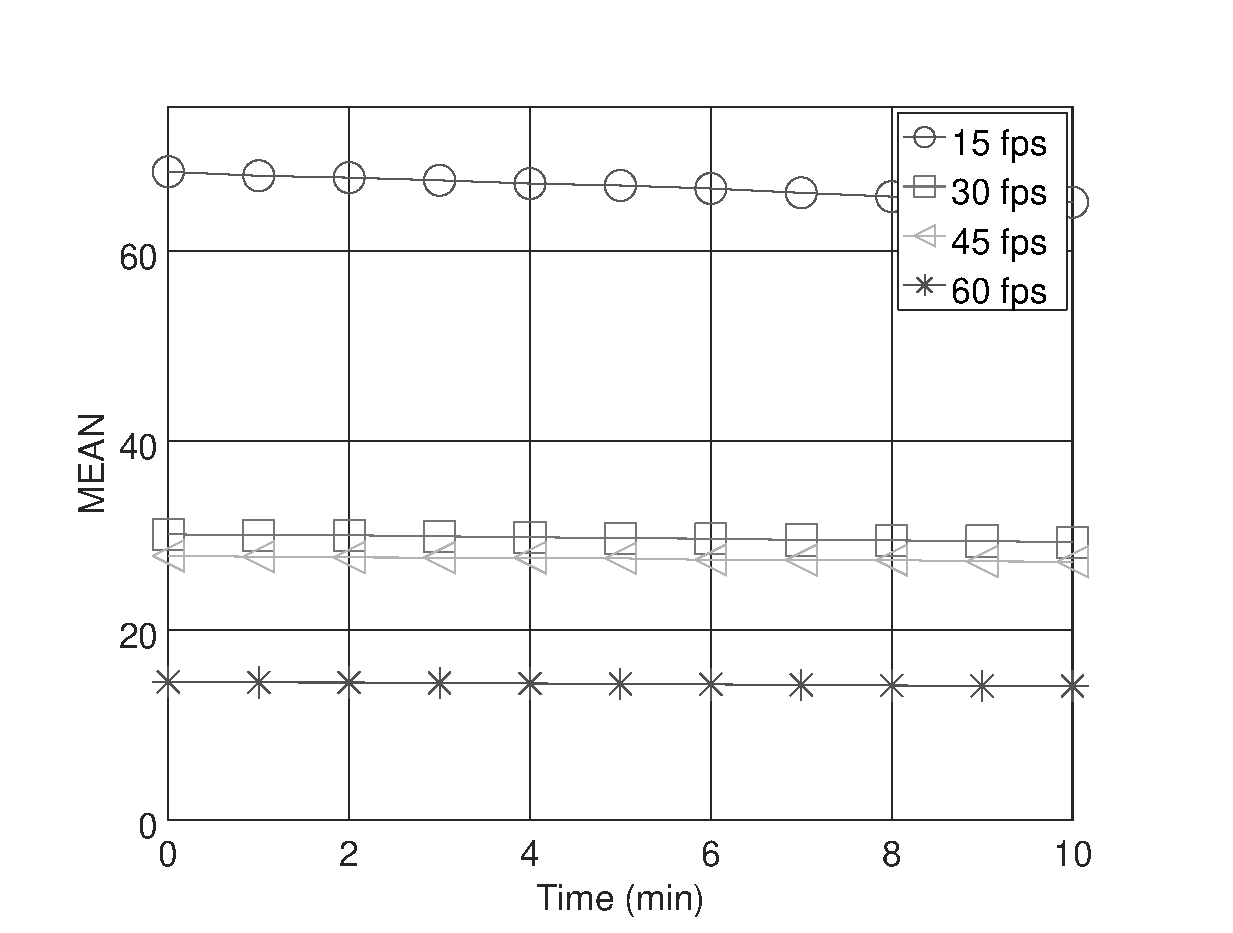
\includegraphics[width=0.5\textwidth]{FPS_f11_rawMEAN.eps}
    \caption{$MEAN$ index value.}\label{fig:MEANtest1}
\end{figure}
It can be seen that, 
the value of index has a monotonous behavior over time. 
By other side the values in the curves decreases in proportion with 
the grow of sampling rate.

%%%%%%%%%%%%%%%%%%%%%%%%%%%%%%%%%%%%%%%%%%%%%%%%%%%%%%%%%%%%%%%%%%%%%%%%%%%%%%%%
Figure \ref{fig:AVDtest1} shows the result of analysis explained in the 
Section \ref{subsec:test1} about the $AVD(t)$ index.
\begin{figure}[ht!]
    \centering
    \begin{subfigure}{0.48\textwidth}
        \caption{$AVD$ index value.}
        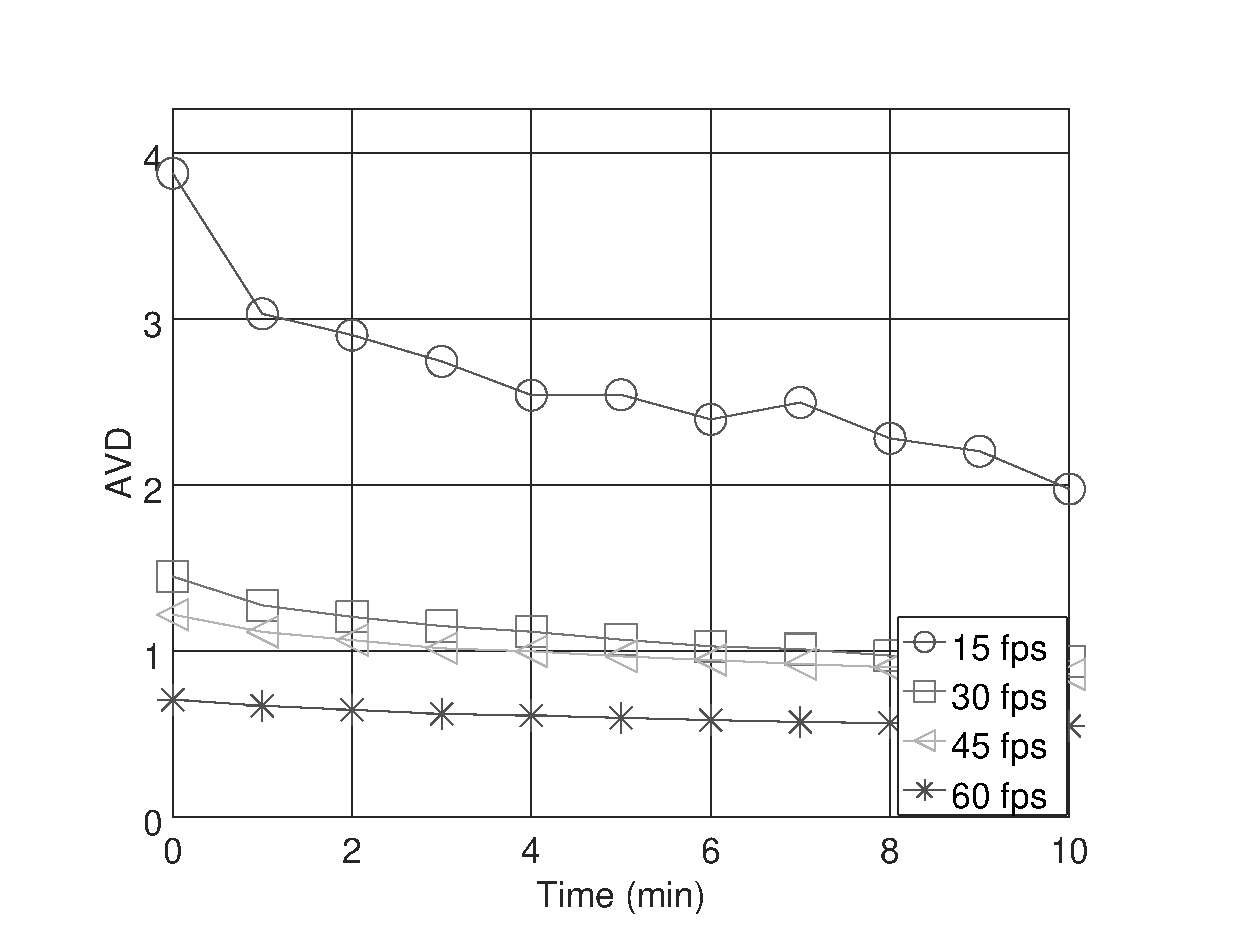
\includegraphics[width=\textwidth]{FPS_f11_rawAVD.eps}
        \label{fig:avdraw}
    \end{subfigure}
    ~ %add desired spacing between images, e. g. ~, \quad, \qquad, \hfill etc. 
      %(or a blank line to force the subfigure onto a new line)
    \begin{subfigure}{0.48\textwidth}
        \caption{Normalized $AVD$ index value.}
        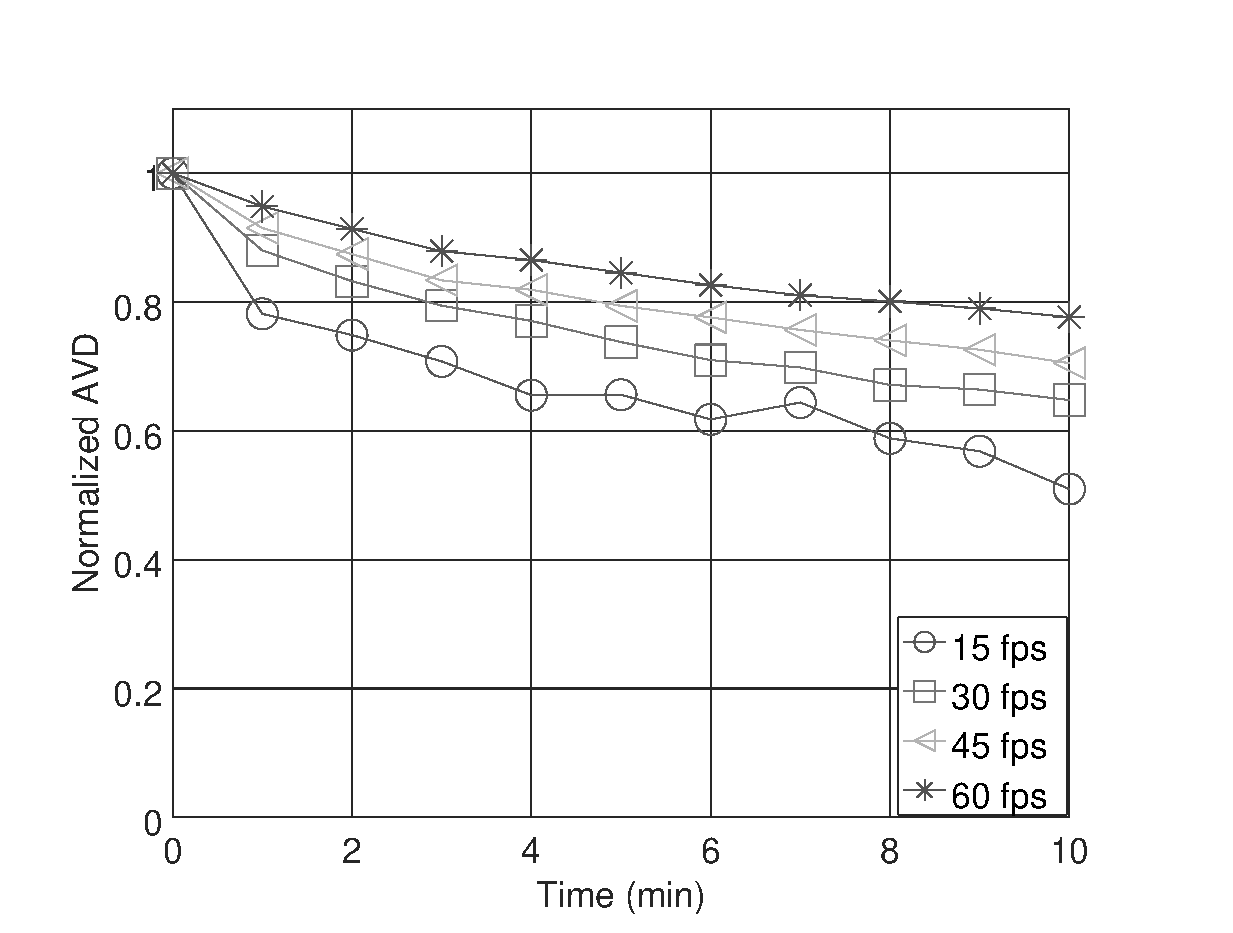
\includegraphics[width=\textwidth]{FPS_f11_norm1AVD.eps}
        \label{fig:avdnorm}
    \end{subfigure}
    \caption{$AVD$ index anaysis.}\label{fig:AVDtest1}
\end{figure}
The Figure \ref{fig:avdraw} shows the $AVD(t)$ index, in each time $t$, 
to 4 sampling rates, showing a different behavior in time to each sampling rate,
so that, the value of the index in all  curves, decreases in proportion with 
the grow of sampling rate. By other side,
Figure \ref{fig:avdnorm} shows a normalized version of $AVD(t)$ index, 
so that the maximum value of curves have an unit value; thus,
it can be seen that, the maximum excursion of the curve is greatest when 
the sampling rate decrease. Remembering that this index uses information from a frequency
band between $F_s/4$ until $F_s/2$ Hz \cite{rivera2017selection}.

%%%%%%%%%%%%%%%%%%%%%%%%%%%%%%%%%%%%%%%%%%%%%%%%%%%%%%%%%%%%%%%%%%%%%%%%%%%%%%%%
Figure \ref{fig:STDtest1} presents the $STD(t)$ index in the test showed in the 
Section \ref{subsec:test1}.
\begin{figure}[ht!]
    \centering
    \begin{subfigure}{0.48\textwidth}
        \caption{$STD$ index value.}
        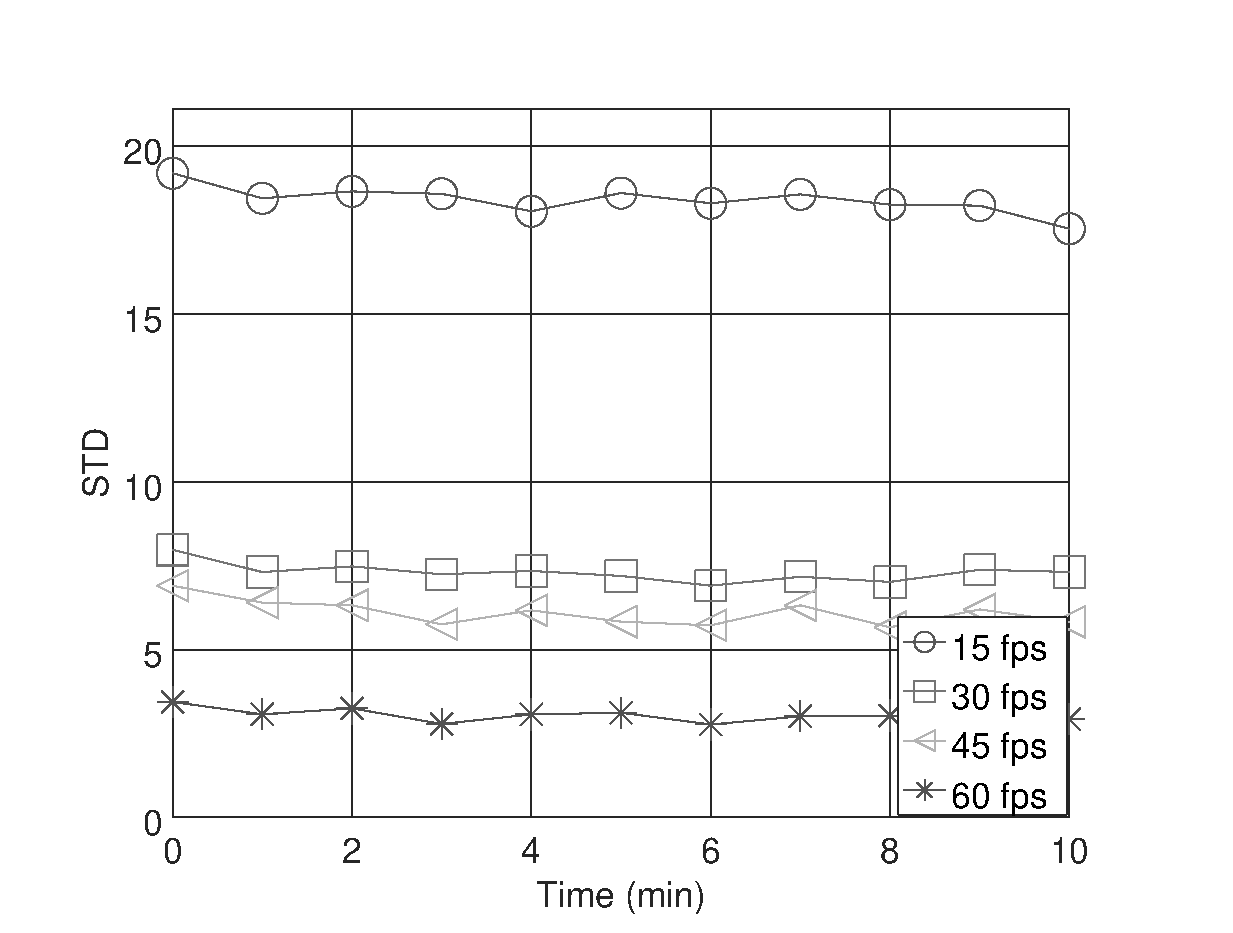
\includegraphics[width=\textwidth]{FPS_f11_rawSTD.eps}
        \label{fig:stdraw}
    \end{subfigure}
    ~ %add desired spacing between images, e. g. ~, \quad, \qquad, \hfill etc. 
      %(or a blank line to force the subfigure onto a new line)
    \begin{subfigure}{0.48\textwidth}
        \caption{Normalized $STD$ index value.}
        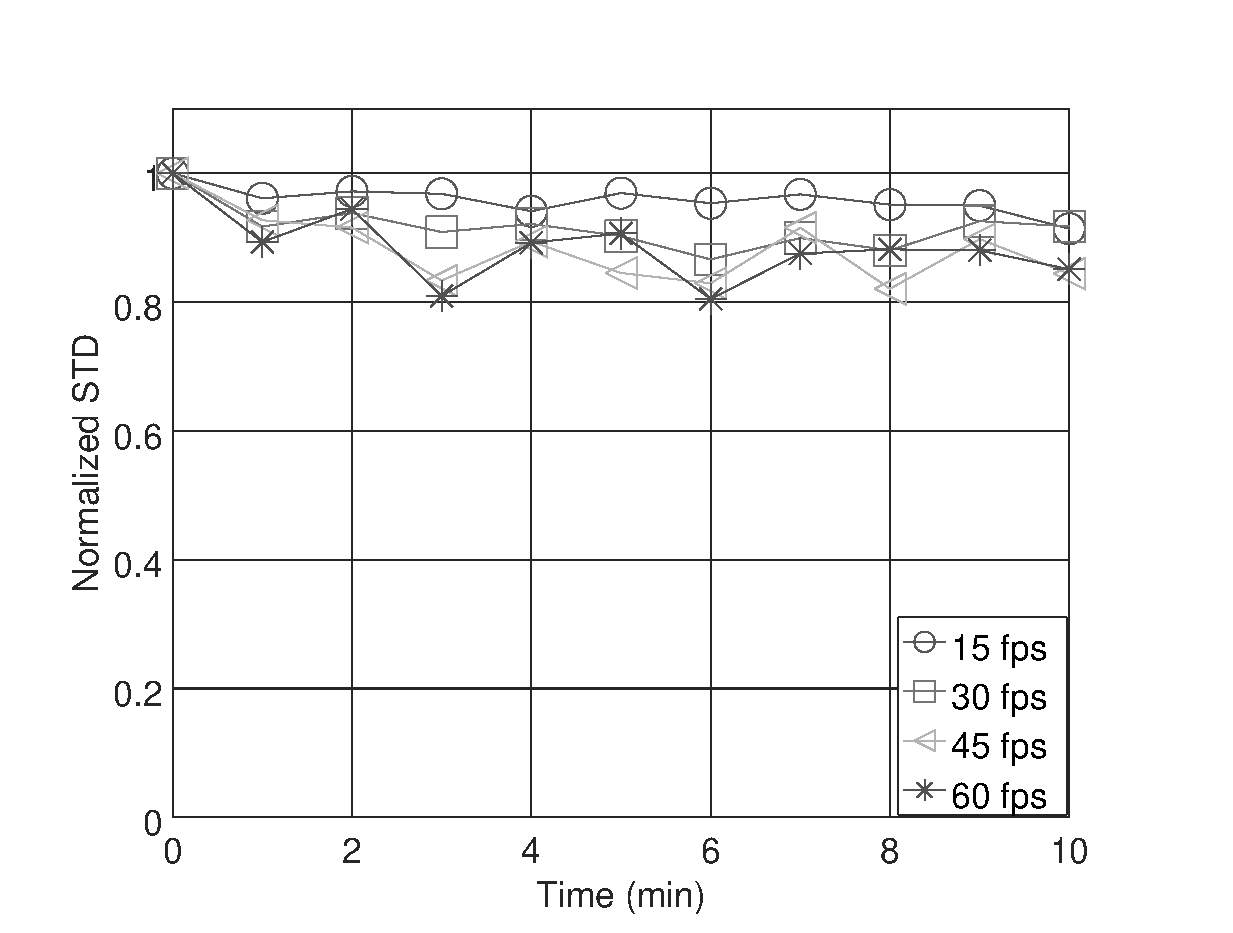
\includegraphics[width=\textwidth]{FPS_f11_norm1STD.eps}
        \label{fig:stdnorm}
    \end{subfigure}
    \caption{$STD$ index anaysis.}\label{fig:STDtest1}
\end{figure}
The Figure \ref{fig:stdraw} shows the  behavior of $STD(t)$ index, in each time $t$, 
to 4 different sampling rates. Remembering that this index uses information in the entire frequency
band ($0$ until $F_s/2$ Hz), as seen in Section \ref{sec:std}.
This index shows a different behavior in time to each sampling frequency,
so that, the value of the index in each time  decreases in proportion with 
the grow of sampling rate. By other side,
Figure \ref{fig:stdnorm} shows a normalized version of $STD(t)$ index;
being the unit, the maximum value of curves; thus,
it can be seen that exists a small difference between the maximum excursion 
of the curves with different sampling rates; even so, it is possible to observe
a slight decrease of the maximum excursion in the curve with the grow of the sampling rate, 
unlike the $AVD(t)$ index.


%%%%%%%%%%%%%%%%%%%%%%%%%%%%%%%%%%%%%%%%%%%%%%%%%%%%%%%%%%%%%%%%%%%%%%%%%%%%%%%%
Figure \ref{fig:STDFtest1}, presents the $STDF(t)$ index, in the test showed in the 
Section \ref{subsec:test1}.
\begin{figure}[ht!]
    \centering
    \begin{subfigure}{0.48\textwidth}
        \caption{$STDF$ index value.}
        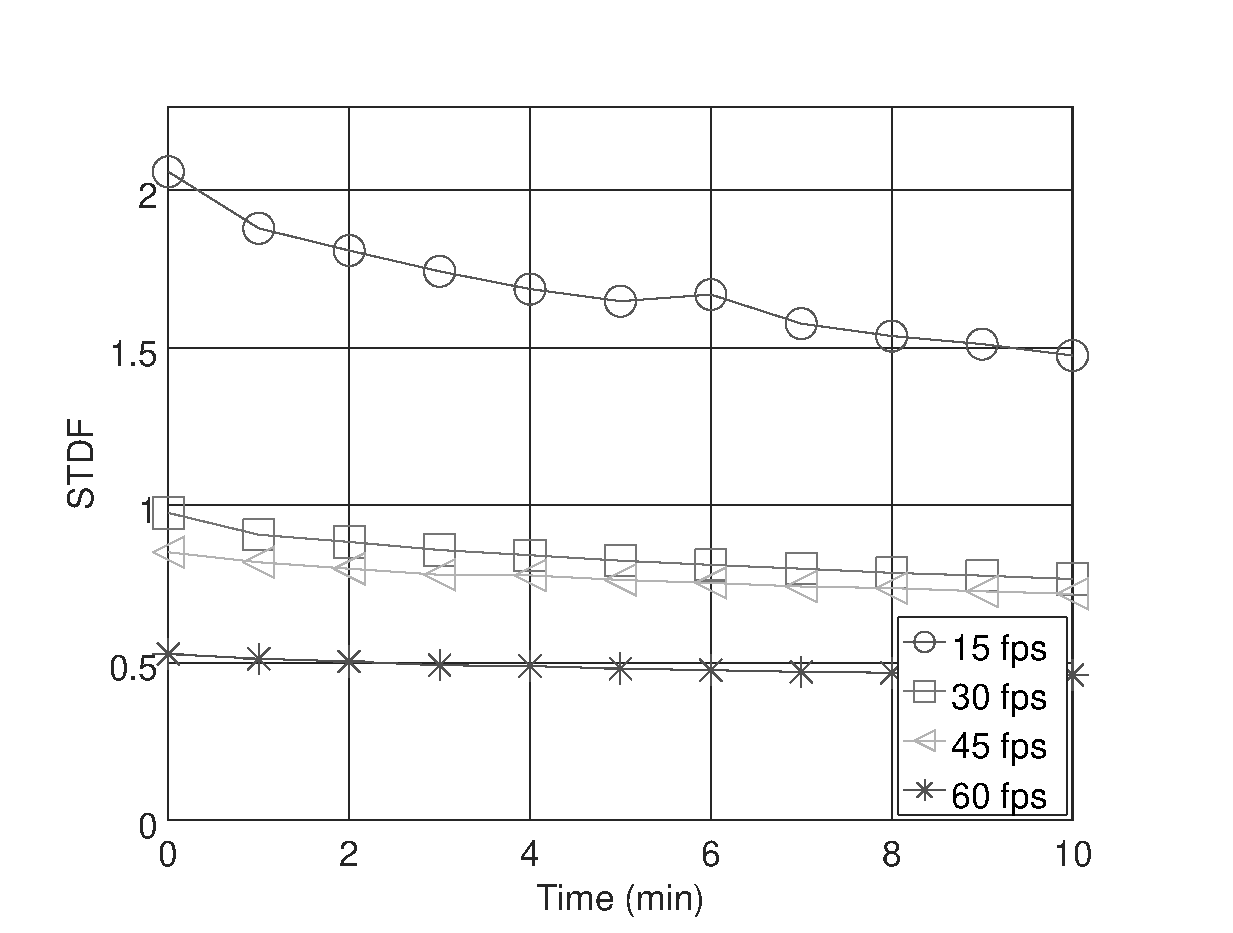
\includegraphics[width=\textwidth]{FPS_f11_rawSTDF.eps}
        \label{fig:stdfraw}
    \end{subfigure}
    ~ %add desired spacing between images, e. g. ~, \quad, \qquad, \hfill etc. 
      %(or a blank line to force the subfigure onto a new line)
    \begin{subfigure}{0.48\textwidth}
        \caption{Normalized $STDF$ index value.}
        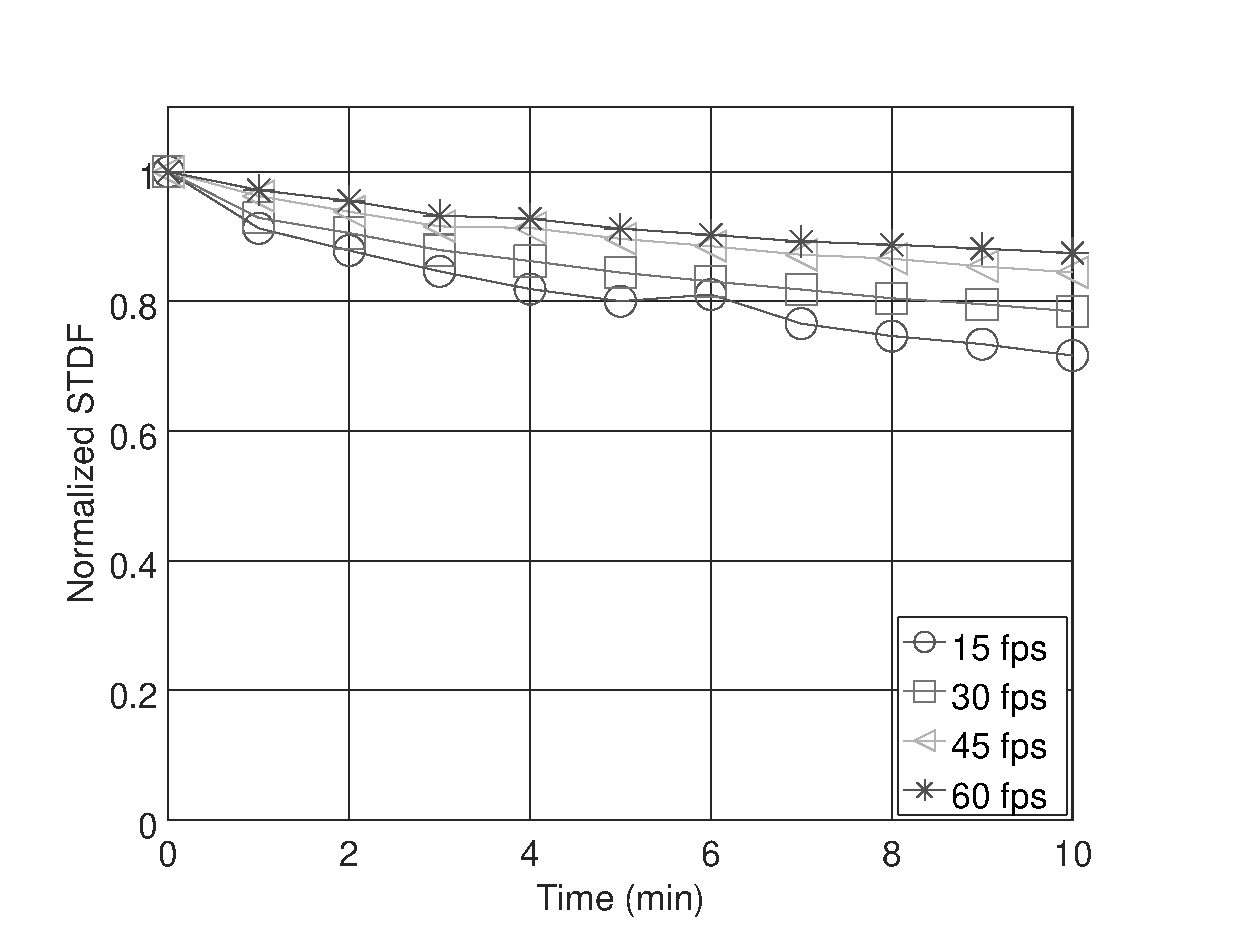
\includegraphics[width=\textwidth]{FPS_f11_norm1STDF.eps}
        \label{fig:stdfnorm}
    \end{subfigure}
    \caption{$STDF$ index anaysis.}\label{fig:STDFtest1}
\end{figure}
Figure \ref{fig:stdfraw} shows the behavior $STDF(t)$ index, in each time $t$, 
to 4 different sampling rates. Remembering that this index uses filtered 
information of datapack, so that the frequency
band is between $F_s/4$ and $F_s/2$ Hz. 
% of similar way of $AVD(t)$ index but with different order filter, as seen in Section \ref{sec:stdf}.
This index shows monotone decreasing behavior in time, where we observe 
a different behavior in time to each different sampling rate;
so that, the value of the index in each time decreases in proportion with 
the grow of sampling rate. By other side,
Figure \ref{fig:stdfnorm} shows a normalized version of $STDF(t)$ index;
being the unit, the maximum value of curves; thus,
it can be seen that exists a considerable difference between the maximum excursion 
of the curves with the use of sampling frequency; so, it is possible to observe a 
grow of the maximum excursion when the sampling rate decrease, like the $AVD(t)$ index.

%%%%%%%%%%%%%%%%%%%%%%%%%%%%%%%%%%%%%%%%%%%%%%%%%%%%%%%%%%%%%%%%%%%%%%%%%%%%%%%%
\subsection{Test 2: maize seed germination}
\label{subsec:resulttest2}

This test shows the result of analyze a corn seed  with 3 days of germination,
the images were taken using the sampling rates: $15$, $30$, $45$ and $60$Hz.

%%%%%%%%%%%%%%%%%%%%%%%%%%%%%%%%%%%%%%%%%%%%%%%%%%%%%%%%%%%%%%%%%%%%%%%%%%%%%%%%
Figure \ref{fig:MEANtest2} shows the $MEAN(t)$ index,
decreasing its value
%in the test described in the Section \ref{subsec:test2};
\begin{figure}[ht!]
    \centering
    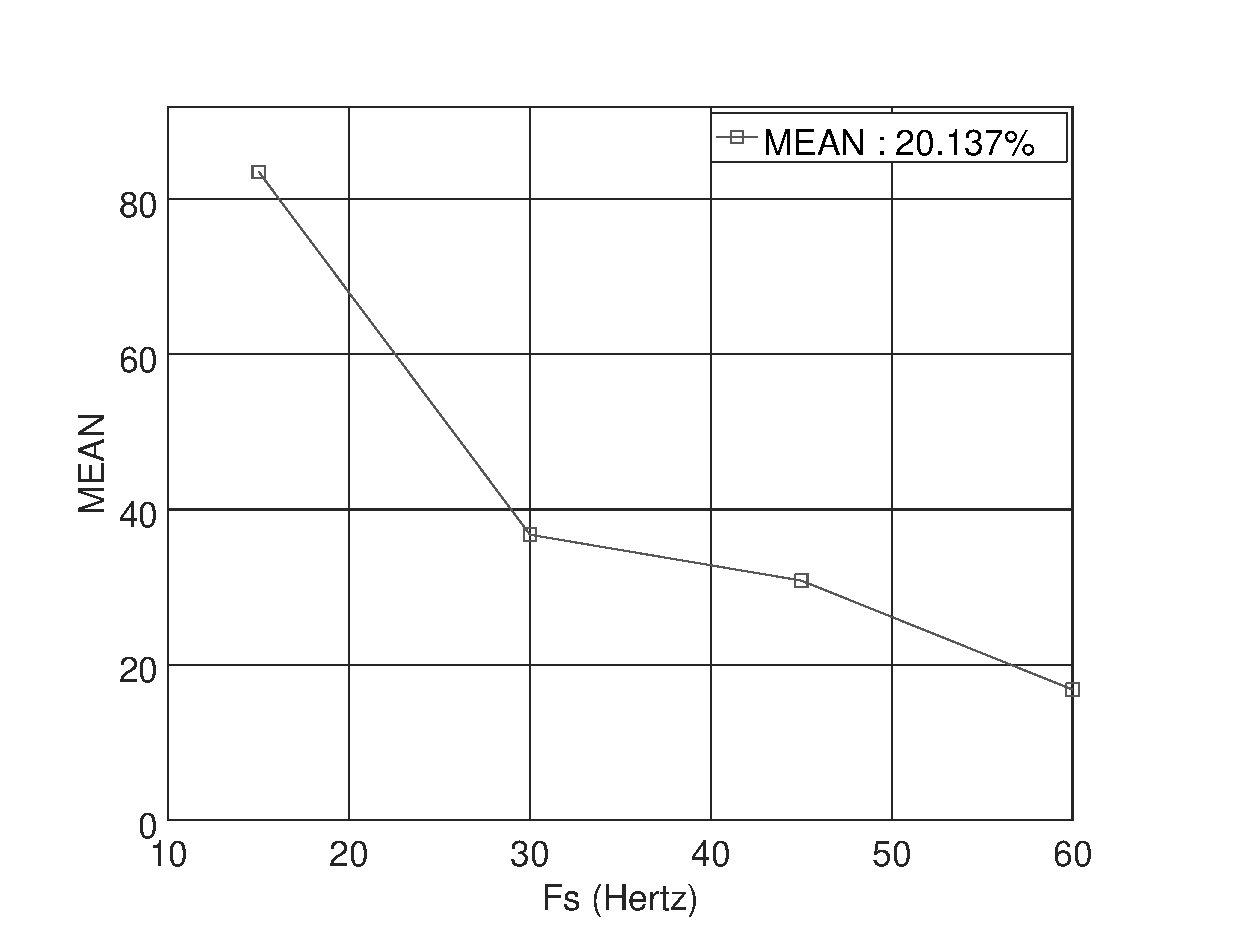
\includegraphics[width=0.5\textwidth]{FPS_Semilla_3_3diasALLMEAN.eps}
    \caption{$MEAN$ index value in the germinated corn seed.}\label{fig:MEANtest2}
\end{figure}
%We observe as the index decrease your value, 
with the increment of sampling frequency, %in the datapack,
where from %so that between 
$15$ Hz to $60$ Hz, the index value reached the $20.137\%$ of its value.


%%%%%%%%%%%%%%%%%%%%%%%%%%%%%%%%%%%%%%%%%%%%%%%%%%%%%%%%%%%%%%%%%%%%%%%%%%%%%%%%
Figure \ref{fig:INDEXtest2} shows the $AVD(t)$, $STD(t)$ and $STDF(t)$ indexes,
with the same behavior that the presented by $MEAN$ index.
%in the test described in the Section \ref{subsec:test2};
\begin{figure}[ht!]
    \centering
    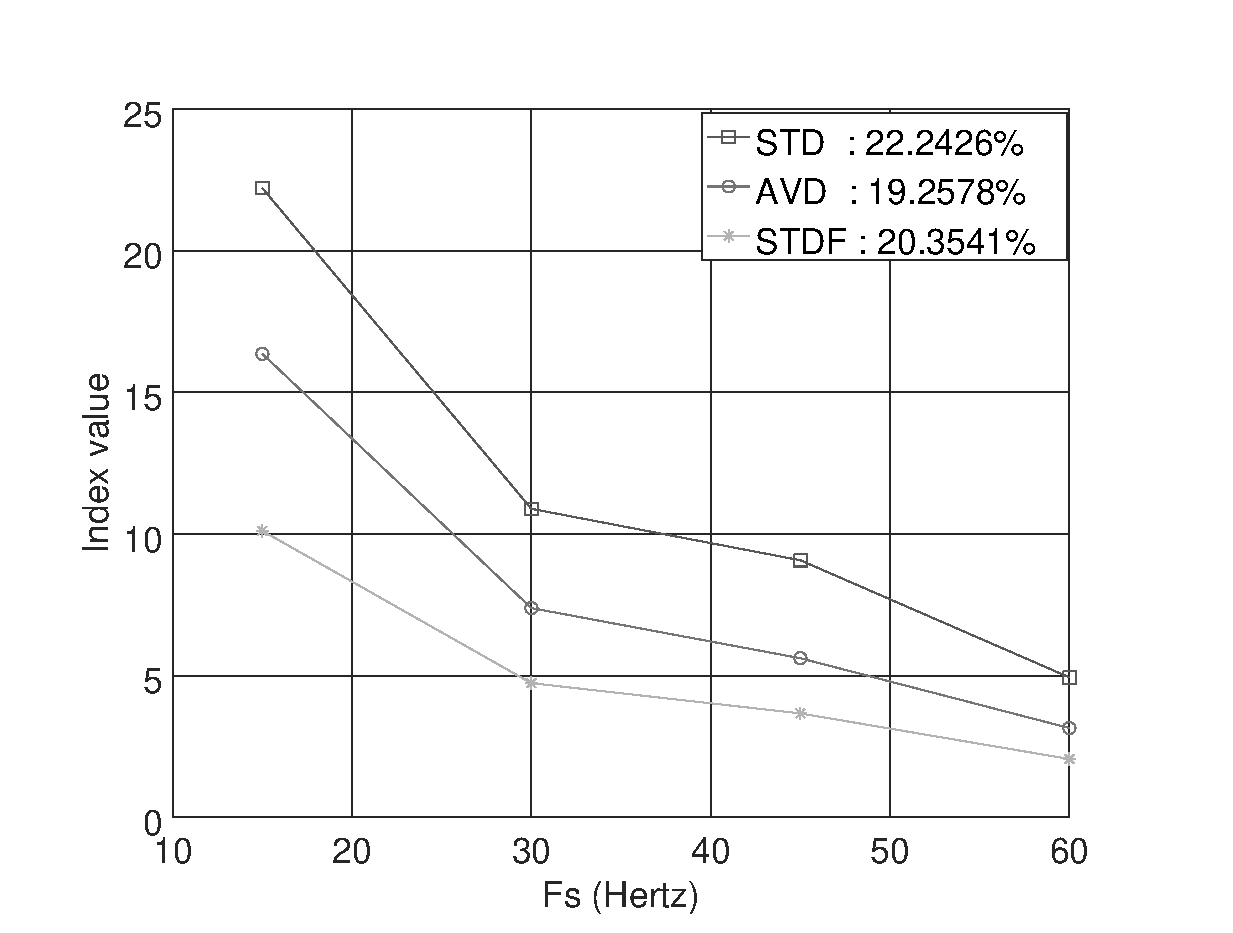
\includegraphics[width=0.5\textwidth]{FPS_Semilla_3_3diasALL.eps}
    \caption{$AVD(t)$, $STD(t)$ and $STDF(t)$ indexes values in the germinated maize seed.}\label{fig:INDEXtest2}
\end{figure}
%The similar way that in the Figure \ref{fig:MEANtest2},
%the index decrease your value with the grow of $F_s$,
%so that the indexes, $STD(t)$, $AVD(t)$  and $STDF(t)$, 
%reaches the $22.2426\%$, $19.2578\%$ and $20.3541\%$ of your values, 
%respectively.
The decreasing of the activity observed are related to the increase of $F_s$
where $STD$, $AVD$ and $STDF$ presented respectively degrowth values of $22.2426\%$
 $19.2578\%$ and $20.3541\%$.
%to highest $F_s$ if compared to the lowest $F_s$.


\subsection{Test 3: frequency band activity analysis}
\label{subsec:resulttest3}
Table \ref{table:2} shows the 
%result of calculating the 
$STDB$ image in different frequency bands 
of maize seed,
%over a package $P$, see Sec. \ref{subsec:test3}, 
%the package represents  a corn seed described in the Section \ref{subsec:data2};
%where, we have packages sampled 
using 4 different sampling rates: $15$, $30$, $45$ and $60$ Hz, as
can be seen in the first column of the table.

%~\\
\begin{table}[h!]
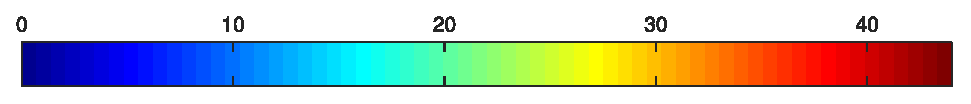
\includegraphics[width=\textwidth]{colorbar.eps}
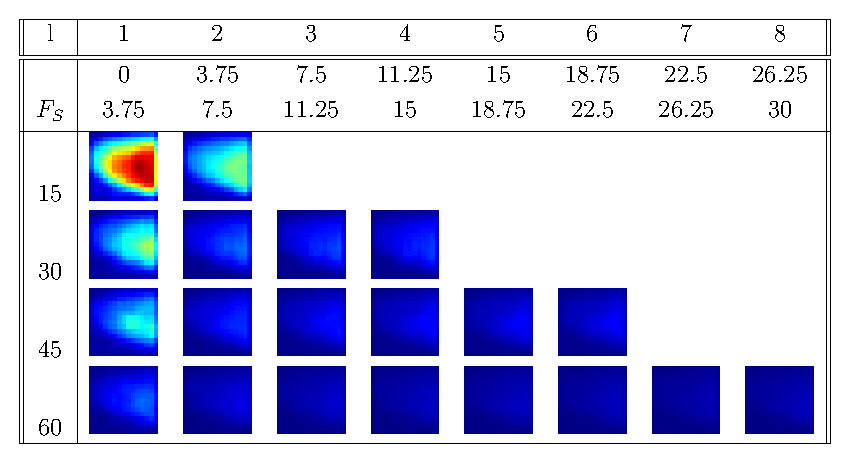
\includegraphics[width=\textwidth]{freq1.eps}
\caption{frequency band analysis}
\label{table:2}
\end{table}
In the other columns, we can see the results of $8$ frequency bands of package $P$,
%these bands are 
represented in the first line of table, with $l$, that indicates the position of frequency band
in crescent order, relative to its frequency components, 
%Thus, we have these frequency bands limited on: 
with limits assigned at the frequencies: $0$, $3.75$, $7.5$, $11.25$, $15$, $18.75$, $22.5$, $26.25$ and $30$Hz;
as can be seen in the second line of table.
So that, the package sampled at $15$hz was divided in $L=2$ frequency bands, 
the package sampled at $30$hz was divided in $L=4$ frequency bands, 
the package sampled at $45$hz was divided in $L=6$ frequency bands and finally
the package sampled at $60$hz was divided in $L=8$ frequency bands.

The matrices $STDB$ are represented using a color palette, 
that goes from dark blue (low values) to dark red color (high values), 
%representing of ascendant way 
linked to the values of activity,
%in each pixel in all matrices, as It is shown in the top of table. 
it is evident how the index values decreases with
the increment of frequency sampling $F_s$.
%in each one of 8 frequency bands, 
The index values also decrease with the increment of the position of frequency band,
being  a frequency band between $0$ Hz and $3.75$ Hz with a sampling rate of $15$ hz,
the better analysis's case; in the sense of better differentiating places of lower and higher index value.




%%%%%%%%%%%%%%%%%%%%%%%%%%%%%%%%%%%%%%%%%%%%%%%%%%%%%%%%%%%%%%%%%%%%%%%%%%%%%%%%
%%%%%%%%%%%%%%%%%%%%%%%%%%%%%%%%%%%%%%%%%%%%%%%%%%%%%%%%%%%%%%%%%%%%%%%%%%%%%%%%
%%%%%%%%%%%%%%%%%%%%%%%%%%%%%%%%%%%%%%%%%%%%%%%%%%%%%%%%%%%%%%%%%%%%%%%%%%%%%%%%
%%%%%%%%%%%%%%%%%%%%%%%%%%%%%%%%%%%%%%%%%%%%%%%%%%%%%%%%%%%%%%%%%%%%%%%%%%%%%%%%
\section{Discussions} 
\label{sec:analysisresults}


%In the results seen in Section \ref{sec:numericalresults}, we can observe in 
In the Figure \ref{fig:MEANtest1} and \ref{fig:MEANtest2}, 
%that 
the indexes show a relation between the profile of mean index curve and the sampling frequency of datapack. 
%How is known \cite{Nothdurft:05}, 
The temporal speckle mean index (Fig. \ref{fig:MEANtest1}) is related to 
the observed illumination level in the surface of the material \cite{Nothdurft:05} and  
correspond to the analysis of zero frequency components of signal.
%correspond to the offset in the frequency domain or frequency zero.
%zero frequency of the signal (datapack);
Thus, we can conclude that the level of illumination, perceived by the camera, 
decrease with the increment of sampling rate. 
This is because that the exposition time is modified with the alteration of sampling frequency to commercial cameras, 
%see Section \ref{subsec:expositiontime}, 
so that less lighting is used to take the picture and consequently the 
temporal speckle mean index decrease in  its value.
In this sense, it is important to be aware to choose a sampling frequency
that gives us an index value superior to the noise level of test or to the quantization level of the camera.


The modification of exposition time also affects  and limits other indexes,
remember that we have a quantization level between $0$ and $255$ in the camera. 
We can see this interference in the Figures \ref{fig:AVDtest1}, \ref{fig:STDtest1}, \ref{fig:STDFtest1} and \ref{fig:INDEXtest2}, 
where the $AVD(t)$, $STD(t)$ and $STDF(t)$ indexes decrease their values in concordance with the decrease of exposition time.
Other way in that  the sampling frequency affects the values of indexes,
can be seen in the limitation of
%It is that, it limits 
the frequency band of an analyzed signal; for example,
a sampling frequency $F_s$, by the Nyquist theorem \cite{Nyquist,Shannon}, 
causes  the limitation of  frequency band %of analyzed signal (datapack)  will be 
between $0 Hz$ and $F_s/2~Hz$.
Thus, in this context we have an index as $STD(t)$ that uses information between $\langle \left. 0, F_s/2 \right ] Hz$, 
while other  indexes as the $AVD(t)$ and the $STDF(t)$ index, use information of half frequency band, 
between $\left [ F_s/4, F_s/2 \right ] Hz$.
In the comparison between $STD(t)$ vs  $\{$ $STDF(t)$ and $AVD(t)$ $\}$, 
we can see how the use of half, of entire frequency band, causes the decrease in the values of the curves, 
but give us considerably good values in the maximum excursion of the curve across the time. By other side,
in the case of ink drying process, the use of complete frequency band ($STD(t)$ index), 
it returns low values of maximum excursion in the curves across the time. 
The importance of excursion, in this test,
 is due to the need of significant differences between the values of two states,
during the
%when the sample start or end the ink 
drying process.

It is necessary to highlight the importance of to choose the best value of sampling rate $F_s$;
so that, 
the frequency band of a signal contain the frequency components with the information that you want to analyze;
so that, the values of indexes have the greatest values and probably a good excursion, 
when compared with an inert part of  the sample. 
By example, in the Table. \ref{table:2}, it is analyzed a corn seed, 
where we can see  the major values of indexes are obtained 
from $0$ Hz and $7.5$ Hz, when $F_s=15$ Hz. 

Thus, at this point,
an question is evident: 
What is the best frequency band? According with the test of corn seed, 
we see that for all frequency bands, 
the best range, 
is the one with the components with lowest possible frequencies; 
but without forget that given a $STD(t)$ analysis, 
this index extract information of inner parts of material \cite{Nothdurft:05}, 
and this information decrease jointly with the decrease of frequency band,
as can be seen when compared the result in the excursion of $STD(t)$, 
with frequency components in low frequencies,
and the excursion of $\{$ $STDF(t)$ and $AVD(t)$ $\}$, 
with frequency components in high frequencies;
so that we need to choose a compromise between the desired quantity of inner information in the sample, 
the perceived illumination level and the sampling rate.

%%%%%%%%%%%%%%%%%%%%%%%%%%%%%%%%%%%%%%%%%%%%%%%%%%%%%%%%%%%%%%%%%%%%%%%%%%%%%%%%
%%%%%%%%%%%%%%%%%%%%%%%%%%%%%%%%%%%%%%%%%%%%%%%%%%%%%%%%%%%%%%%%%%%%%%%%%%%%%%%%
%%%%%%%%%%%%%%%%%%%%%%%%%%%%%%%%%%%%%%%%%%%%%%%%%%%%%%%%%%%%%%%%%%%%%%%%%%%%%%%%
%%%%%%%%%%%%%%%%%%%%%%%%%%%%%%%%%%%%%%%%%%%%%%%%%%%%%%%%%%%%%%%%%%%%%%%%%%%%%%%%
\section{Conclusion} 

In this work were presented comparisons of three dynamic laser speckle indexes,
subject to different values of sampling rate.
thus we conclude that it is important to choose an appropriate sampling rate, 
being recommendable to use the minimal sampling frequency possible to get an acceptable maximum excursion, 
in index as the $AVD$ and $STDF$,
and an illumination level in the images with good signal-noise relation,
so that the phenomenon under study can be collected in the chosen analysis frequency band.
We showed that the digitization  of speckle signal imply a restriction of frequency 
band of signal and consequently this affect the result of an speckle analysis.
And the user of a digital camera must be aware that the increase of the frame rate (fps) 
force the commercial cameras to change the perceived illumination level in the camera sensor.

%%%%%%%%%%%%%%%%%%%%%%%%%%%%%%%%%%%%%%%%%%%%%%%%%%%%%%%%%%%%%%%%%%%%%%%%%%%%%%%%
%%%%%%%%%%%%%%%%%%%%%%%%%%%%%%%%%%%%%%%%%%%%%%%%%%%%%%%%%%%%%%%%%%%%%%%%%%%%%%%%
%%%%%%%%%%%%%%%%%%%%%%%%%%%%%%%%%%%%%%%%%%%%%%%%%%%%%%%%%%%%%%%%%%%%%%%%%%%%%%%%
%%%%%%%%%%%%%%%%%%%%%%%%%%%%%%%%%%%%%%%%%%%%%%%%%%%%%%%%%%%%%%%%%%%%%%%%%%%%%%%%
\section{Acknowledgment}
We wish to acknowledge the partial financial support for this study provided by the $CAPES$ 
scholarship
$PNPD$ Program, $FAPEMIG$ and $CNPQ$.


%%%%%%%%%%%%%%%%%%%%%%%%%%%%%%%%%%%%%%%%%%%%%%%%%%%%%%%%%%%%%%%%%%%%%%%%%%%%%%%%
%%%%%%%%%%%%%%%%%%%%%%%%%%%%%%%%%%%%%%%%%%%%%%%%%%%%%%%%%%%%%%%%%%%%%%%%%%%%%%%%
%%%%%%%%%%%%%%%%%%%%%%%%%%%%%%%%%%%%%%%%%%%%%%%%%%%%%%%%%%%%%%%%%%%%%%%%%%%%%%%%
%%%%%%%%%%%%%%%%%%%%%%%%%%%%%%%%%%%%%%%%%%%%%%%%%%%%%%%%%%%%%%%%%%%%%%%%%%%%%%%%
\section{Bibliography}
\bibliography{report}   %>>>> bibliography data in report.bib
\bibliographystyle{spiebib}   %>>>> makes bibtex use spiebib.bst


\end{document} 


